%Dokumentinnstillinger:---------------------------------
%Ved å google flitting kan du finne ut hva de forskjellige tingene her betyr, og hvordan du kan gjøre eventuelle endringer.
\documentclass[a4paper,11pt,norsk]{article}
\usepackage[utf8]{inputenc}
\usepackage{a4wide}
\usepackage{lmodern}
\usepackage[T1]{fontenc}
\usepackage{babel}
\usepackage{textcomp}

\setlength{\parindent}{0pt} 
\setlength{\parskip}{2ex}
\usepackage{fixltx2e}
\usepackage{amsmath}
\usepackage[pdftex, pdfborderstyle={/S/U/W 0}]{hyperref}
\usepackage{graphicx}
\usepackage[font=small,labelfont=bf]{caption}
\usepackage{tabularx}
\usepackage{multirow}
\usepackage{circuitikz}
% Adds seperation between two elements with a comma. Format: "    ,    ".
\newcommand{\comma}{\quad , \quad}
% Gives double underline under selected text.
\def\dunderline#1{\underline{\underline{#1}}}
% Faster way to make an equation that can be formatted with "&" to look nice.
\def\spliteq#1{\begin{equation}\begin{split}{#1}\end{split}\end{equation}\\}
%------------------------------------- End -------------------------------------

\begin{document}

%Headingdel:---------------------------------------------
\begin{minipage}[c]{0.15\textwidth}

\includegraphics[width=2.0cm]{Design_projects/elsys_pos_staaende_ntnu.png}
\end{minipage}
\begin{minipage}[c]{0.85\textwidth}

\renewcommand{\arraystretch}{1.7}
\large 
\begin{tabularx}{\textwidth}{|X|X|}
\hline
\multicolumn{2}{|l|}{} \\
\multicolumn{2}{|l|}{\huge \textbf{Designnotat 1}} \\
\multicolumn{2}{|l|}{}  \\
\hline
\multicolumn{2}{|l|}{Tittel: 
%Skriv inn tittel her:------------------------------------------
Frekvensmultiplikator (ulineært delsystem)
} \\
\hline
\multicolumn{2}{|l|}{Forfattere: 
%Skriv inn forfattere her:--------------------------------------
Sindre Danielsen
} \\
\hline
%Skriv inn versjon og dato her her:-----------------------------
Versjon: 3.0 & Dato: 09.06.21
\\
\hline 
\end{tabularx}
\end{minipage}
\normalsize

%Automatisk generert innholdsfortegnelse:------------------

\setlength{\parskip}{0ex}
\renewcommand{\baselinestretch}{0.1}\normalsize
\tableofcontents
\renewcommand{\baselinestretch}{1.00}\normalsize
\setlength{\parskip}{2ex}
\rule{\textwidth}{1pt}

%Selve rapporten:----------------------------------------÷
\newpage
\section{Problembeskrivelse}
\label{sec:innledning}
Det finnes tilfeller der frekvensøkning av en krets er ønskelig. Det kan da brukes et system vist ved figur~\ref{fig:frekvensdobler_generell}.
\begin{figure}[htbp]
    \centering
    \begin{circuitikz} [american voltages, european resistors, baseline=(current bounding box.center)]
        \ctikzset { label/align = straight }
        \draw (2.5,2)
        to[short, -o] (4,2)
        to[short] (4.5,2)
        (4, 1.6) to [open,v=$\mathbf{x(t)}$] (4,0.4)
        % Bottom-left side
        (2.5,0) to[short, -o] (4,0)
        to[short] (4.5,0)
        %Top between systems
        (8.5,2) to[short] (10,2)
        %Bottom between systems
        (8.5,0) to[short] (10,0)
        % Top-right side
        (15.5,2) to[short, -o] (14.5,2)
        to[short] (14, 2)
        (14.5, 1.6) to [open,v=$\mathbf{\hat{s}(t)}$] (14.5,0.4)
        % Bottom-right side
        (15.5, 0) to[short, -o] (14.5,0)
        to[short] (14,0);
        
        % Nivåregulator
        \node[draw,minimum width=4cm,minimum height=3.8cm,anchor=south west] at (4.5,-0.90){\textbf{Ulineært  system}};
        \node[draw,minimum width=4cm,minimum height=3.8cm,anchor=south west] at (10,-0.90){\textbf{Båndpass filter}};

        
    \end{circuitikz}
    \caption{Frekvensmultiplikator: $f_{\hat{s}} = k \cdot f_{x}$}
  \label{fig:frekvensdobler_generell}
\end{figure} \\
Inngangsignalet $\mathbf{x(t)}$ representerer utgangsignalet $\mathbf{\hat{s}(t)}$ med en økt frekvens $f_{\hat{s}}$, gitt av \\ multiplikatorkonstanten $k$ og frekvensen av $x(t)$ som er $f_x$.
\\\\
Det anbefales å oppnå en så stor Q-faktor (engelsk: Quality factor) som mulig. Se seksjon~\ref{sec:prinsipielllosning} for mer informasjon.

\newpage
\section{Prinsipiell løsning}
\label{sec:prinsipielllosning}
For å endre frekvensen til et inngangsignal, så brukes et ulineært system for å lage et \\frekvensspekter. En slik krets er vist ved figur~\ref{fig:ulin_system}.
\begin{figure}[htbp]
    \centering
    \begin{circuitikz} [american voltages, european resistors, baseline=(current bounding box.center)]
        \ctikzset { label/align = straight }
        \draw (0, 0)
        % Diode
        to[short,o-] (1,0)
        to[empty diode, l=$D$,-o] (4,0)
        % Resistor av diode
        to[resistor, l=$R$,-o] (4,-2)
        
        
        % Out of circuit
            % Top
        (4,0) to[short,-o] (6,0)
            % Bottom
        (0,-2) to[short,o-o] (6,-2)
        
        % Signals
            % In
        (0, -0.2) to [open,v=$\mathbf{v_{in}(t)}$] 
        (0,-1.8)
            % Out
        (6, -0.2) to [open,v=$\mathbf{v_{out}(t)}$] (6, -1.8)
        
        ;
        
        % Dashed box
        \node[draw,dashed,minimum width=4cm,minimum height=3.75cm,anchor=south west] at (1,-2.75);

        
    \end{circuitikz}
    \caption{Dannelse av frekvenspekter, der $v_{in}$ har en konstant frekvens.}
  \label{fig:ulin_system}
\end{figure} \\
Det brukes en diode $D$ og motstand $R$, samt inngangsignal $v_{in}$ og utgangssignal $v_{out}$. \\\\

Vi selekterer den ønskede frekvensen på utgangen $\hat{s}(t)$ ved bruk av et båndpassfilter, der med en frekvens $f_{\hat{s}}$:
\begin{equation}
   f_{\hat{s}} = \frac{\omega_0}{2\pi}. 
\end{equation}
\\
Resonnansfrekvensen gir oss verdiene for kretsen: \\
\begin{equation}
    f_{\hat{s}} = \frac{1}{2\pi \sqrt{C\cdot L}} 
    \quad \implies \quad 
    L = \frac{1}{2\pi f_{\hat{s}}^2 \cdot C} 
    \comma 
    C = \frac{1}{2 \pi f_{\hat{s}}^2 \cdot L}
\end{equation}\label{eq: resonnans}
$C$ er kapasitansen og $L$ er induktansen for båndpassfilteret.
\\\\
Dette gjelder for enhver motstandverdi i båndpassfilteret, men for et optimalt båndpassfilter så kreves en maksimal Q-faktoren $Q$ er bestemt av båndpassfilterets komponenter:
\begin{equation}
    Q = \sqrt{\frac{L}{CR_{min}^2}},
    \label{eq:q-faktor}
\end{equation}
der $R_{min}$ er den laveste motstandsverdien til båndpassfilteret, uten at det forstyrrer signalet til en vesentlig grad. Lave motstandsverdier vil forstyrre signalet, det beste er å teste seg frem.
\\
\\
Q-faktor er en måling på kvaliteten på et båndpassfilter. Visuelt er det vist på den øverste grafen i figur~\ref{fig: frekvensspekter}, der vi ønsker en grafen så høy og spiss som mulig. 

\\
I tillegg så anbefales det å bruke buffer mellom det ulinære systemet og båndpassfilteret. Også mellom hvert båndpassfilter. En buffer en en op-amp med med sin negative pol koblet til utgangen på op-ampen. Der den positive polen tar inn det signalet, som ønskes.
Bufferens mål er å sørge for at tidligere kretselement ikke påvirker neste kretselement og omvendt. Gjelder både spenning og strøm.

\newpage
\section{Realisering og test}
\label{sec:realisering}
Verdiene brukt i realiseringen av frekvensmultiplikatoren er vist ved tabell~\ref{table:variabler}.
\\
\begin{table}[htbp]
\centering
\begin{tabular}{ |c|c|c|c| } 
\hline
\textbf{Navn} & \textbf{Verdi} & \textbf{Beskrivelse}\\
\hline
$f_x$ & $2.8$kHz & Frekvens inngangssignal $x(t)$.  \\
\hline
$k$ & 2 & Valgt frekvensmultiplikator. \\
\hline
$L$ & $0.2$H & Teoretisk spole\\
\hline
$R$ & $1000 \Omega$ & Teoretisk valgt motstand.  \\ 
\hline
$C$ & $4$nF & Gitt av likning~\ref{eq: resonnans} \\ 
\hline
$R_{min}$ & $150$ & Ekperimentelt funnet motstandsverdi \\
\hline
$D$ & 1N4733A & Zenerdioden (5.1V) \\
\hline
$R$ & $1$k$\Omega$ & Eksperimentelt funnet motstand \\
\hline
$Q$ & 47.1 & Q-faktor (likning~\ref{eq:q-faktor})\\
\hline
\end{tabular}
\caption{Verdiene brukt i realisering av systemet.}
\label{table:variabler}
\end{table}
\\
For den oppkoplede kretsen, se figur~\ref{fig: realKrets}. \\\\
Målingen av frekvensspekteret for $\hat{s}$ er vist ved 
\begin{figure}[htbp]
\centering
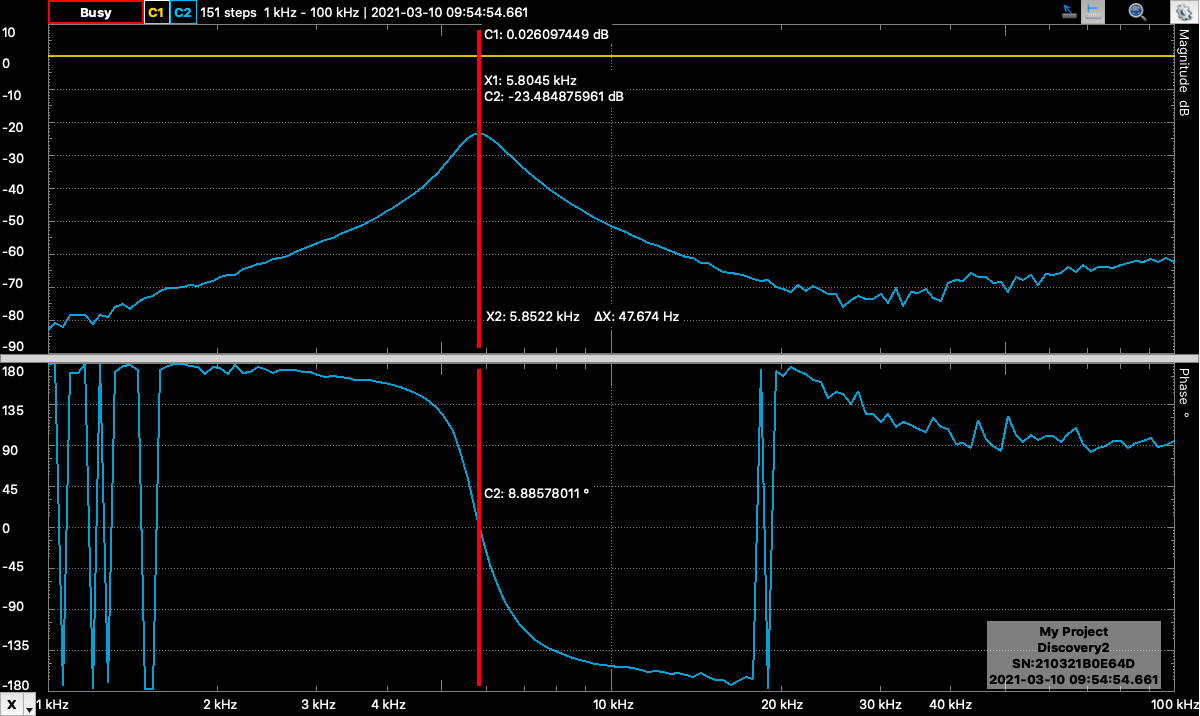
\includegraphics[width=1.0\textwidth]{img/Network_Waveforms_img.png}
\caption{Observert frekvensspekter av $\hat{s}(t)$.}
\end{figure}\label{fig: frekvensspekter}
\\
der den gule funksjonen er $x(t)$ og den blå $\hat{s}$. Grafavbildningen øverst gjelder for amplituden til en hver frekvens av signalene, mens den nederste grafavbildningen er faseforskyvningen.  \\\\\\
Figur~\ref{fig: frekvensspekter} viser et båndpassfilter med korrekt oppførsel, for nesten korrekt frekvens. \\
Mulig avvik fremkommer av at kapasitansen og/eller induktansen avviker fra de antatte \\verdiene. \\
Verdt å merke seg at spenningsfallet ved resonnansfrekvensen avviker fra den teoretetiske modellen av et båndpassfilter. Det vil alltid være en viss mengde av spenningsfall over andre komponenter i kretsen.
\newpage
Figur~\ref{fig: frekvensspekter} viser en tilnærmet frekvensdobling på utgangssignalet, som også kan observeres ved å sammenlikne $x(t)$ og $\hat{s}$ for $f_{\hat{s}}$, slik vist i
\begin{figure}[htbp]
\centering
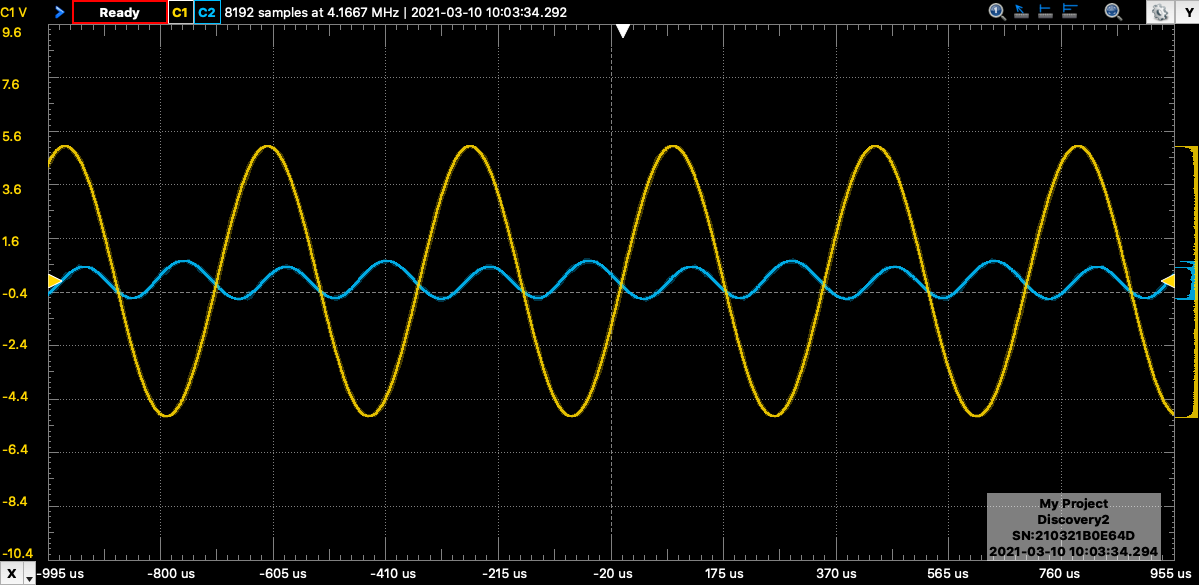
\includegraphics[width=1.0\textwidth]{img/Scope_Waveforms_img.png}
\caption{Waveforms: Gul graf $x(t)$, blå graf $\hat{s}$, for $f_{\hat{s}}$}
\label{fig: realKrets}
\end{figure}
\\
Her fremkommer også konsekvensene av et ulineært system. Ikke bare vil frekvensen bli endret, men amplituden er vesentlig mindre, samt en liten faseforskyvning.
\newpage
\begin{figure}[htbp]
\centering
\includegraphics[width=1.0\textwidth]{img/20210310_115718.jpg}
\caption{Reell krets av figur~\ref{fig:frekvensdobler_generell}.}
\label{fig: realKrets}
\end{figure}
I den oppkoblede kretsen er det valgt å kaskadekopling to båndpassfiltre, som vil gi en god nok oppførsel på $\hat{s}(t)$.



\newpage
\section{Konklusjon}
\label{sec:konklusjon}
Systemet som er utviklet fra figur~\ref{fig:frekvensdobler_generell} har tatt i bruk et ulineært system, som påvirker amplituden, faseforskyvningen og frekvensen til $\hat{s}(t)$. Det er vist i seksjon~\ref{sec:realisering} at systemet fungerer som en frekvensmultiplikator. For et bedre frekvensspekter for figur~\ref{fig: frekvensspekter}, så kan det kaskadekoples flere båndpassfiltre (Seriekoble båndpassfiltre med buffer imellom).
Det kan også velges større induktans eller lavere kapasitans i båndpassfilteret, slik at Q-faktoren blir større. Unngå å sette motstandsverdien $R_{min}$ for lav, fordi fare for ustabilt signal.
\newpage



%Bibliografi: Legg til flere elementer ved å legge til flere \bibitem:--------

\appendix 
\section{Vurdering}
\begin{itemize}
\item Generelt ser teksten ut til å være kort og presis.
\item Figurene gir en god nok representasjon av av det som forklares i seksjonen den gjelder.
\item Uvisst om notatet er en besvarelse på en oppgave eller ikke.
\item Symbol og variabler er representert og avbildet på en god måte.
\item Figurer blir forklart.
\item Figurer og formler er nummerert og har korrekt variabelbruk.
\item Det refereres godt til tidligere deler av teskten ved behov for det.
\end{itemize}

\section{Ønsker tilbakemelding på}
Forstod jeg var litt ''pratete'' på D2, så har forsøket å redusere på det.
Usikker på om jeg skriver for lite nå.\\
\\
Antok at siden vi skal skrive til andre på ''samme nivå'' som oss, så setter jeg ikke opp kretsen for båndpassfilter og kaskadekopling, siden det er selvforklarende hvordan dette ser ut, siden det er tidligere pensum. Tenker jeg riktig da?
\\
Hvis oppgaven fremdeles bærer preg av å være en ''besvarelse'', så hadde et par eksempler der det forekommer vært fint. Fordi sliter litt med å se det selv.
\\
\\
Er det nødvendig å ha med realisert kretsdesign til slutt, selv om oppsettet er godt forklart og egentlig bare er likt som i figur~\ref{fig:frekvensdobler_generell} men med ett ekstra båndpassfilter? Liksom antar ikke at inmaten er viktig å formidle i realisering, når man allerede vet hvordan det ulineære systemet og båndpassfiltrene ser ut inni.
\\\\
Er det tilstrekkelig nok de grafene i figurene, eller er det nesten et must å plotte det i python? Tenkte det var litt unødvendig siden det vil vise grafene på en lik måte som i WaveForms.

%Tillegg. Flere tillegg legges til ved å lage flere sections:-----------------
\end{document}